%   ------------------------------------------------------------------------
\FloatBarrier
\section{Análise do RosebudAI}

A ferramenta RosebudAI foi selecionada por demonstrar ter foco na criação de sprite sheets, especificamente para jogos. Na sua página inicial (Figura \ref{fig:rosebudInicial} no Apêndice \ref{ap.telasIA}), afirmações como "Use IA para criar sprites para seu jogo" apontavam para a capacidade da plataforma em criar animações para um personagem. No entanto, a análise revelou uma ferramenta com múltiplas funcionalidades que, em todos os testes, falhou em produzir um sprite sheet 2D consistente a partir de uma imagem de referência. 

Os testes foram realizados em junho, focando no ambiente principal da plataforma. O objetivo principal era produzir o sprite sheet ou animação do walking cycle (ciclo de caminhada, em inglês) do personagem utilizando o sprite de Pablo em front view (apresentado anteriormente na Figura \ref{fig:Pablo}). Na primeira tentativa, em vez de um sprite sheet, a ferramenta apresentou um protótipo de jogo 3D, incluindo um script de 600 linhas de código (interação completa pode ser consultada na Figura \ref{fig:rosebud1} do Apêndice \ref{ap.telasIA}). O personagem gerado (Figura \ref{fig:rosebudJogo} manteve vagamente as cores da referência, porém com um estilo cúbico inadequado, em uma aparente tentativa de emular o estilo pixel art em um ambiente tridimensional.

\begin{figure}[htbp]
    \centering
    \caption{\small Resultado do teste inicial}
    \label{fig:rosebudJogo}
    \begin{subfigure}{0.3\linewidth}
        \centering
        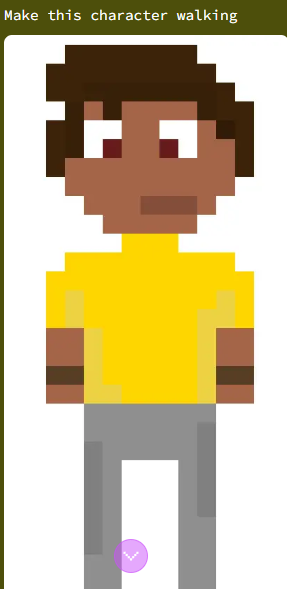
\includegraphics[width=1\linewidth]{figs/rosebud/principal1.PNG}
        \caption{\small Prompt e imagem de referência.}
        \label{fig:rosebudJogoPrompt}
    \end{subfigure} \hfill
        \begin{subfigure}{0.65\linewidth}
        \centering
        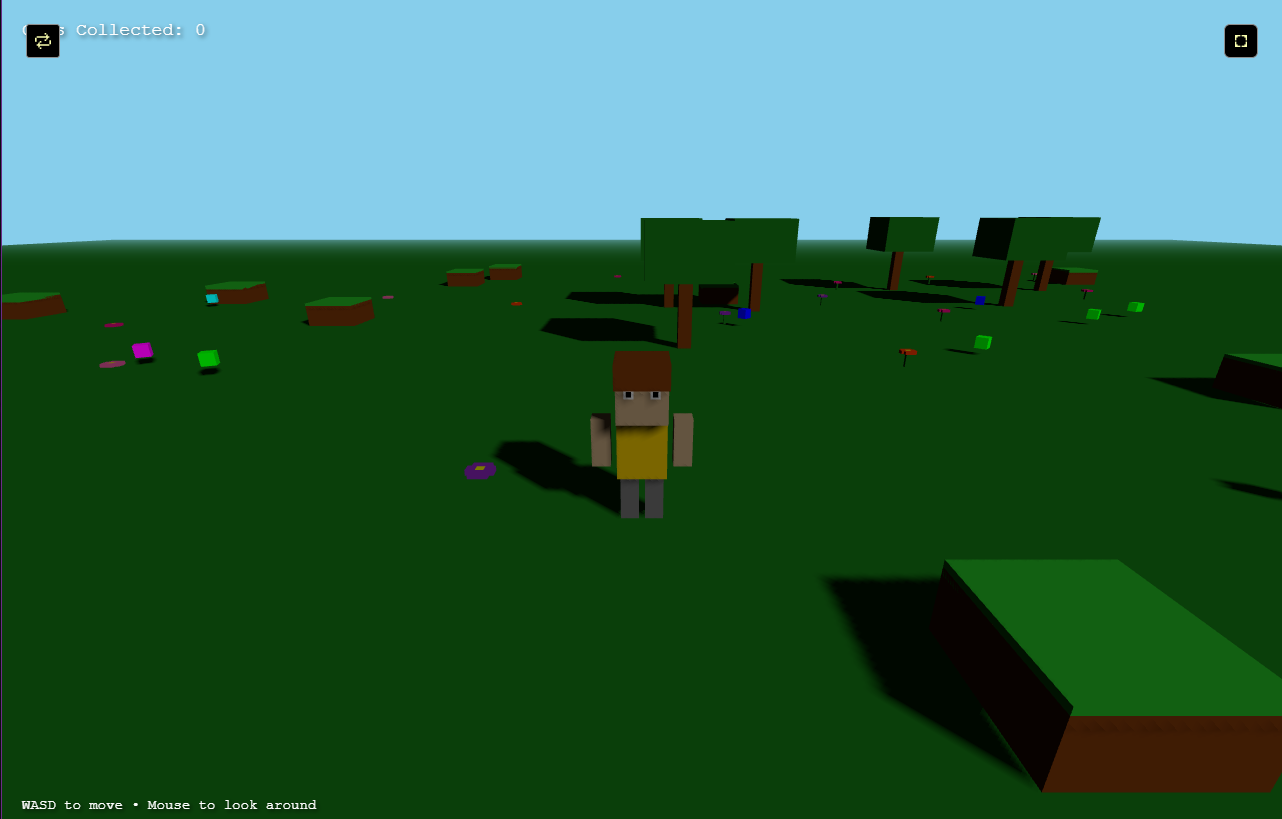
\includegraphics[width=1\linewidth]{figs/rosebud/principal2.PNG}
        \caption{\small Interface do jogo gerado.}
        \label{fig:rosebudJogoJogo}
    \end{subfigure}

    \legend{\small Fonte: Elaborada pela autora.}
\end{figure}


Em uma tentativa subsequente, com um prompt ajustado para especificar um cenário 2D e manter a consistência do personagem, a ferramenta produziu uma animação de baixa qualidade\footnote{https://drive.google.com/file/d/1yPtpKDM2CYCaxSqFJr3NFbVswduzkfTY/view?usp=sharing}, na qual metade da imagem de referência é apenas deslocada horizontalmente pela tela, alternando entre a parte inferior ou superior visível na tela, como é demonstrado na Figura \ref{fig:rosebudAnimacao}. A análise dos quadros revelou que  a IA interpretou a imagem de referência como se fosse um sprite sheet completo de dois quadros, dividindo-a ao meio e alternando entre as metades superior e inferior. As imagens completas desse teste podem ser consultadas na Figura \ref{fig:rosebud2} no Apêndice \ref{ap.telasIA}.

\begin{figure}[htbp]
    \centering
    \caption{\small Animação gerada pelo Rosebud AI}
    \label{fig:rosebudAnimacao}
    
    \begin{subfigure}{0.45\linewidth}
        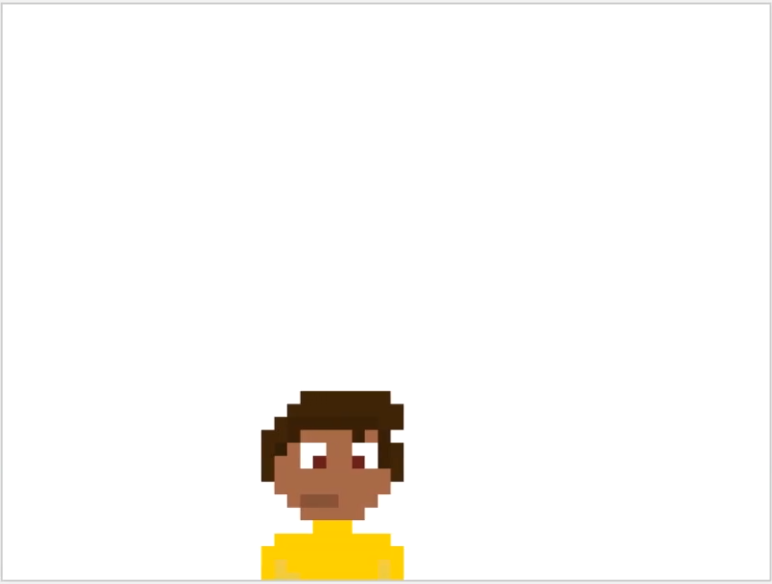
\includegraphics[width=1\linewidth]{figs/rosebud/rosebud_resultado_tela3_1.PNG}
        \caption{\small Frame 1 (metade superior).}
        \label{fig:rosebudFrame1}
    \end{subfigure}
    \begin{subfigure}{0.45\linewidth}
        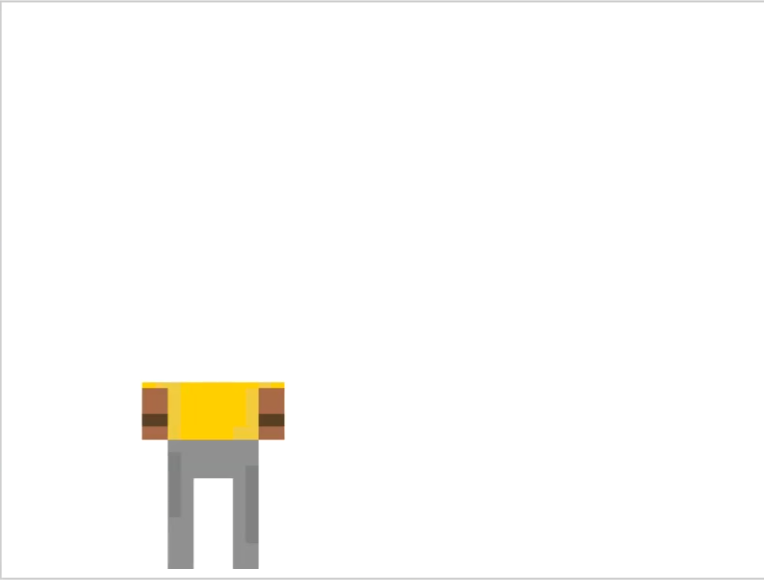
\includegraphics[width=1\linewidth]{figs/rosebud/rosebud_resultado_tela3_2.PNG}
        \caption{\small Frame 2 (metade inferior).}
        \label{fig:rosebudFrame2}
    \end{subfigure}

    \legend{\small Fonte: Elaborada pela autora, utilizando a ferramenta Rosebud AI.}
\end{figure}

Diante desse resultado, os prompts foram ajustados para especificar a criação de um sprite sheet do personagem em várias posições diferentes. Após algumas interações sem sucesso no ambiente principal, que podem ser consultadas na Figura \ref{fig:rosebud3} no Apêndice \ref{ap.telasIA}, a análise foi direcionada para uma seção separada dedicada à geração de assets (Figuras \ref{fig:rosebudPrincipal} e \ref{fig:rosebudAssets} no Apêndice \ref{ap.telasIA}). O primeiro teste nesta seção resultou na geração de um sprite único que desconsiderou completamente a imagem de referência, criando um personagem novo em um estilo distinto.

Com os testes voltados para a área de assets (interação completa mostrada pelas Figuras \ref{fig:rosebud4} no Apêndice \ref{ap.telasIA}), a ferramenta específica para geração de imagens demonstrou desconsiderar a imagem de referência, apresentando um personagem completamente novo em um estilo distinto. Além disso, foi gerado apenas um sprite em vez do sprite sheet do personagem andando. A tentativa de refinar os prompts, utilizando a IA principal para descobrir como referenciar a imagem corretamente, também levou a resultados insatisfatórios. Conforme demonstrado na Figura \ref{fig:rosebudResultadosFinais}, os sprite sheets gerados apresentaram falhas graves, como a mudança do cenário e inconsistência entre os quadros, além de ainda desconsiderar a referência. A documentação completa destes testes se encontra nas Figuras \ref{fig:rosebud4} e \ref{fig:rosebud5} do Apêndice \ref{ap.telasIA}.

\begin{figure}[htbp]
    \centering
    \caption{\small Resultados finais}
    \label{fig:rosebudResultadosFinais}
    \begin{subfigure}{0.45\textwidth}
    \caption{\small Sprite sheet com cenário mudando e frames faltando}
    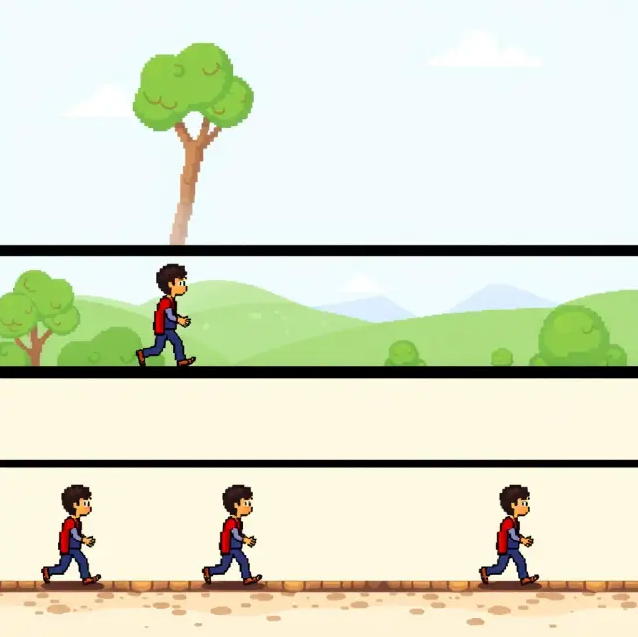
\includegraphics[width=1\linewidth]{figs/rosebud/rosebud_resultado_tela7.PNG}
    \label{fig:rosebudSpriteSheetFrameFaltando}

    \end{subfigure}\hfill
    \begin{subfigure}{0.45\textwidth}
    \caption{\small Sprite sheet com frames inconsistentes entre si}
    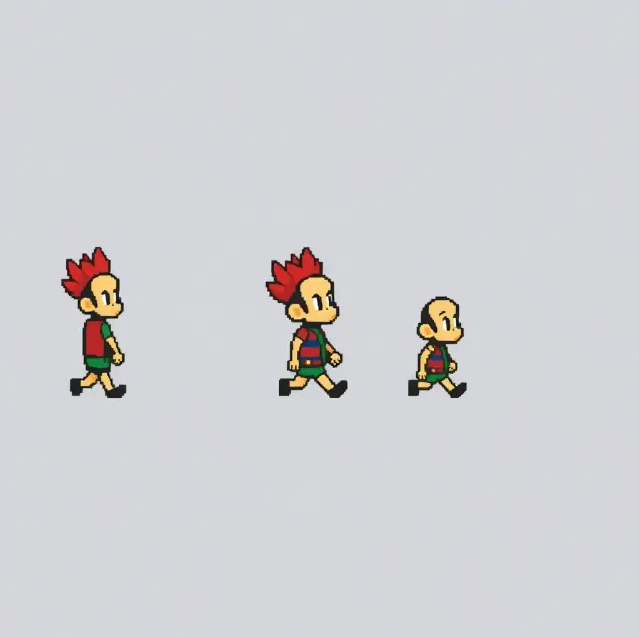
\includegraphics[width=1\linewidth]{figs/rosebud/rosebud_resultado_tela8.PNG}
    \label{fig:rosebudSpriteSheetInconsistente}
    \end{subfigure}\hfill
    \legend{\small Fonte: Elaborada pela autora, utilizando a ferramenta Rosebud AI.}
\end{figure}


Considerando que nenhuma das abordagens produziu um resultado satisfatório, a ferramenta foi descartada para esse estudo. Embora não seja viável para a criação de animações 2D personalizadas, a plataforma  demonstra potencial para a prototipagem rápida de jogos simples para usuários que não possuem conhecimento em programação.
